\documentclass[a4paper,12pt]{article} 

%%% Работа с русским языком
\usepackage{cmap}                           % поиск в PDF
\usepackage{mathtext} 			 	       % русские буквы в формулах
\usepackage[T2A]{fontenc}               % кодировка
\usepackage[utf8]{inputenc}              % кодировка исходного текста
\usepackage[english,russian]{babel}  % локализация и переносы

%Матеша
\usepackage{amsmath,amsfonts,amssymb,amsthm,mathtools} % AMS
\usepackage{icomma} % "Умная" запятая
\usepackage{float}

%\mathtoolsset{showonlyrefs=true} % Показывать номера только у тех формул, на которые есть \eqref{} в тексте.

%% Шрифты
\usepackage{euscript}	 % Шрифт Евклид
\usepackage{mathrsfs} % Красивый матшрифт

%% Свои команды
\DeclareMathOperator{\sgn}{\mathop{sgn}}

%% Перенос знаков в формулах (по Львовскому)
\newcommand*{\hm}[1]{#1\nobreak\discretionary{}
{\hbox{$\mathsurround=0pt #1$}}{}}

%%% Заголовок
\author{Морозов Александр}
\title{Лабораторная работа 2.4.1

Определение теплоты испарения жидкости}
\date{\today}

\begin{document}
	
\maketitle 
	
	
\newpage





\section{Теоретическая справка}

\begin{figure}[h]	\label{plan1}
	\center{\includegraphics[width= 0.5\linewidth]{IMG_1.jpg}}
	\caption{Экспериментальная установка}
\end{figure}	
В данной работе я вычислил теплоту испарения жидкости двумя способами:
\begin{enumerate}
    \item Используя формулу Клапейрона-Клаузиуса
    \begin{equation} \label{kk}
 \dfrac{dP}{dT}= \dfrac{L}{T(V_2 - V_1)}. 
\end{equation}

В дальнейшем для вычислений будут использованы величины из данной таблицы

\begin{center}
\begin{tabular}{|l|*{6}{c|}} 
	\hline
	& $T_{кип}$,&$ V_1$, &$ V_2 , $&$ b$,& $ a$, & $a / V^2$, \\
	   &  & $10^{-6}$ &$10^{-3}$&$10^{-6}$&& \\
	& К &$\frac{м^3}{моль} $&$\frac{м^3}{моль} $&$\frac{м^3}{моль} $&$\frac{Па \cdot м^6}{моль^2} $ &кПа\\ 
	\hline 
	Вода & 373 & 18 & 31 & 26 & 0,4& 0,42 \\ 
        \hline
	\end{tabular}
\end{center}
 Можем пренебречь величиной $V_1$ по сравнению с $V_2$ (далее просто $V$)

\item Другой способ, более точный. В нем используется уравнение Ван-дер-Ваальса
\begin{equation} \label{vv}
\left(P + \dfrac{a}{V^2}\right)\left(V - b\right)= RT.
\end{equation}
Слагаемыми $\frac{a}{V^2}$ и $b$ можем пренебречь, так как при давлениях ниже атмосферного они будут вносить незначительную ошибку, так что:
\begin{equation} \label{ig}
V = \frac{RT}{P}.
\end{equation}
Подставляя \eqref{ig} в \eqref{kk}, пренебрегая $V_1$ и разрешая уравнение относительно $L$, найдём 
\end{enumerate}
Таким образом
\begin{equation} \label{res}
L = \frac{RT^2}{P}\frac{dP}{dT}=-R\frac{d(\ln P)}{d(1/T)}
\end{equation}
Эта формула является окончательной. 
Остальные неизвестные найдем как угловой коэфицент касательной к графикам

\section{Вычисления и обработка данных}
\subsection{Получение экспериментальных данных}
Последовательно повышая, а затем понижая температуру измерим уровни жидкости в обоих менисках, и температуру на датчике. 
По разности уровней жидкости рассчитаем давление, используя формулу $P = \rho_{рт} g \Delta h$. По полученным данным построим графики в координатах $T$,  $P$  и в координатах $1/T$,  $\ln P$ .

Опираясь на экспериментальные данные построим два графика:
\begin{enumerate}
    \item График зависимости Давления от Температуры
    
\begin{figure}[H!]	
	
	\center{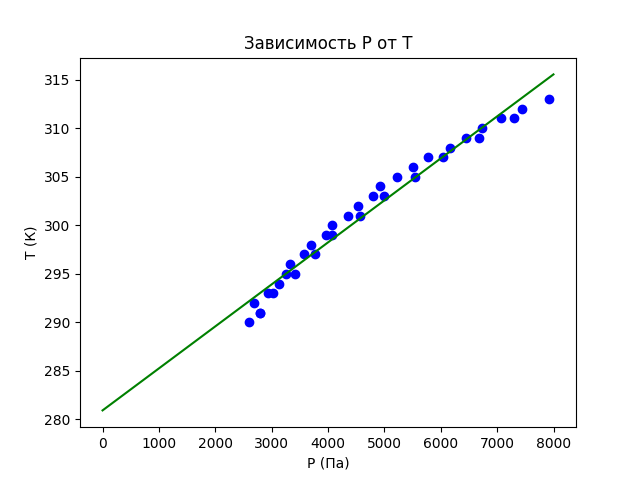
\includegraphics[width= 0.7\linewidth]{function_graph.png}}
\end{figure}
    
    \item График зависимости $ln(P)$ от $\frac{1}{T}$
    
\begin{figure}[H!]	
	
	\center{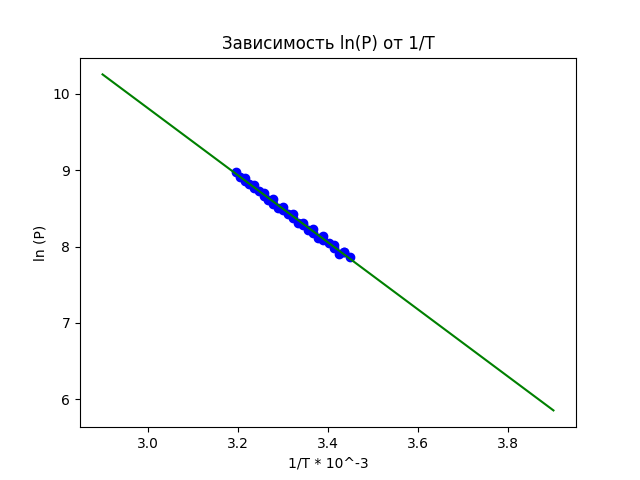
\includegraphics[width= 0.7\linewidth]{ln_graph.png}}
\end{figure}
\end{enumerate}

\subsection{Вычисление L первым способом}

По формуле \eqref{res} вычислим $L$.

Вычислим наклон касательной в середине параболы. Посчитаем L в нескольких точках по формуле (1).
\begin{table}[h!] 
	\caption{Вычисление коэффициента $L$}
	\begin{center}
		\begin{tabular}{|*{9}{l|}}
			\hline 
		
				$T$,$^{\circ}$C & 22&	23&	24&	25&26& 27 &28 &29 \\ \hline
				$L$, кДж/кг& 2123 & 2415 & 2498 & 2217& 2349 & 2314& 2572 & 2537 \\ \hline
				
		\end{tabular}
		
	\end{center}
\end{table}

Подсчитаем статистическую погрешность: $  \sigma _{ст}L\approx 0,3 МДж/кг$, то есть  
$$L = (2,4 \pm 0,3) МДж  / кг$$

\newpage
\subsection{2-ой способ} Воспользуемся вторым графиком. Теплота вычисляется как наклон апроксимирующей прямой, домноженной на коэфицент, так что тут все проще. Не забываем также про статистическую погрешность штангенциркуля и термометра.  

$$
L =( 2,33 \pm 0,05) МДж/кг 
$$

Табличное значение: L = 2,13 МДж/кг

\section{Вывод}


Измерение теплоты испарения вторым способ показало более высокую точность, так как в нем используется метод наименьших квадратов для прямого вычисления, в то время как в первой способе для точных(или не очень) вычислений нужно брать много дополнительных экспериментальных точек. Также во втором случае при вычислении задействуется меньше измеряемых величин, а значит точность выше.


\end{document}


